Im Folgenden werden Mockups präsentiert, welche das Design und die Benutzer\-ober\-fläche der PONG App darstellen. Kleinere Änderungen an Design und der Benutzer\-ober\-fläche während des Entwicklungsprozesses sind möglich.

\subsubsection{Figure 17 - Icon Legende}
Figure \ref{fig:dia:icons} listet die in der App verwendeten Icons auf.
\vspace*{0.5cm}

\begin{figure}[h!]
    \begin{center}
        \begin{tabular}{ll}
            
\includegraphics[width=1.5em,height=1.5em]{diagramme/assets/Media-Play-256.png} & Start / Fortsetzen \\
            
\includegraphics[width=1.5em,height=1.5em]{diagramme/assets/Media-Pause-256.png} & Pause \\
            
\includegraphics[width=1.5em,height=1.5em]{diagramme/assets/Close-256.png} & Beenden\\
            
\includegraphics[width=1.5em,height=1.5em]{diagramme/assets/Arrow-Left-05-256.png} & Zurück \\
            
\includegraphics[width=1.5em,height=1.5em]{diagramme/assets/Floppy-256.png} & Speichern und Fortfahren \\
            
\includegraphics[width=1.5em,height=1.5em]{diagramme/assets/Money-Coin-02-WF-256.png} & Coins / Kontostand \\
            
\includegraphics[width=1.5em,height=1.5em]{diagramme/assets/Heart-256.png} & Symbolisiert ein Leben \\
            
\includegraphics[width=1.5em,height=1.5em]{diagramme/assets/Globe-256.png} & Sprachauswahl \\
            
\includegraphics[width=1.5em,height=1.5em]{diagramme/assets/Shirt-256.png} & Allgemeines Symbol für Skins \\
            
\includegraphics[width=1.5em,height=1.5em]{diagramme/assets/list.png} & Top-10 Liste \\
            
\includegraphics[width=1.5em,height=1.5em]{diagramme/assets/Trophy-256.png} & Achievements \\
            
\includegraphics[width=1.5em,height=1.5em]{diagramme/assets/Bomb-256.png} & Beispiel für \gls{powerup}-Block \\    
            
\includegraphics[width=1.5em,height=1.5em]{diagramme/assets/Lock-256.png} & Item gesperrt / nicht im Besitz
        \end{tabular}
    \end{center}
    \captionof{figure}{Icon Legende}\label{fig:dia:icons}
\end{figure}
\setlength{\extrarowheight}{0.5em}

\clearpage

\subsubsection{Dialog u00 - Hauptmenü}\label{dialog:hauptmenu}

\begin{figure}[h!]
    \begin{center}
    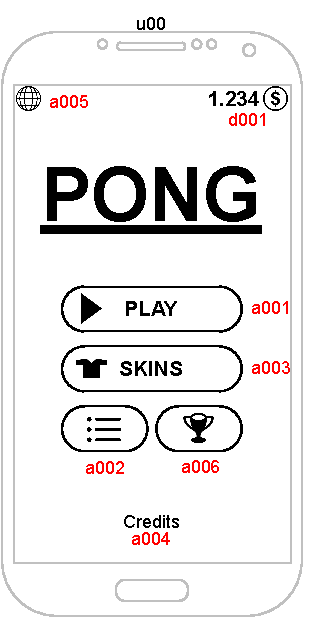
\includegraphics[scale=1.4]{diagramme/pdf/Mockup-u00.pdf}
    \end{center}
    \captionof{figure}{Dialog u00 - Hauptmenü}\label{fig:dia:u00}
\end{figure}

Das Hauptmenü dient dem \gls{spieler} als Ausgangspunkt. Von hier aus kann es möglich sein, die Sprache zu ändern (a005) und die persönlichen Achievements einzusehen (a006). 
Außerdem muss der \gls{spieler} die Anzahl seiner \glspl{coin} ablesen können (d001). Der Play-Button muss den \gls{spieler} zu den Spielmodus Einstellungen führen (a001).
Um die Skin-Auswahl zu öffnen (a003), muss der \gls{spieler} den Skins-Button drücken. Die Top-10 Liste muss sich über den Top-10-Button öffnen lassen (a002). Informationen über das Entwicklerteam muss der \gls{spieler} 
über den Credits-Button abrufen können (a004).
(siehe Fig. \ref{fig:dia:u00})

\clearpage

\subsubsection{Dialog u01 - Spielmodus Einstellungen}\label{dialog:einstellungen}

\begin{figure}[h!]
    \begin{center}
    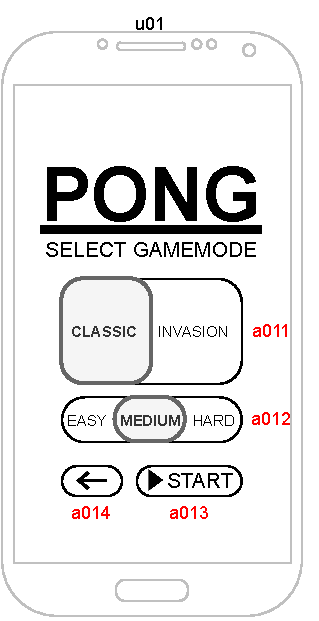
\includegraphics[scale=1.4]{diagramme/pdf/Mockup-u01.pdf}
    \end{center}
    \caption{Dialog u01 - Spielmodus Einstellungen}\label{fig:dia:u01}
\end{figure}

Möchte der \gls{spieler} ein Spiel starten, so muss es zunächst eine Auswahl zwischen den Spielmodi \gls{classicMode} und \gls{invasionMode} geben (a012). Nach der Wahl des Spielmodus muss der \gls{spieler} einen der drei Schwierigkeitsstufen (a011) wählen können.
Zurück zum Hauptmenü muss der \gls{spieler} mit dem Zurück-Button gelangen. Wenn der \gls{spieler} seine Entscheidungen über Spielmodus und Schwierigkeitsstufe getroffen hat, muss das Spiel mit dem Start-Button gestartet werden können.
(siehe Fig. \ref{fig:dia:u01})
\clearpage

\subsubsection{Dialog u02a - Spiel Classic}\label{dialog:classic}

\begin{figure}[h!]
    \begin{center}
    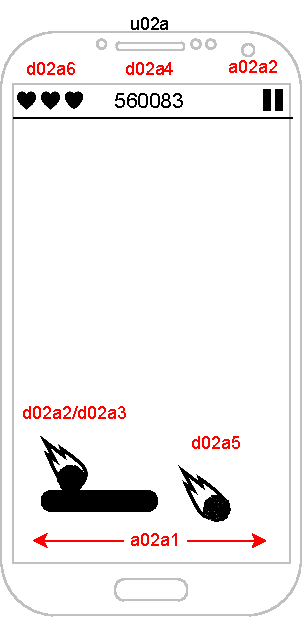
\includegraphics[scale=1.4]{diagramme/pdf/Mockup-u02a.pdf}
    \end{center}
    \caption{Dialog u02a - Spiel Classic}\label{fig:dia:u02a}
\end{figure}

Der Screen "Spiel Classic" muss neben dem beweglichen \gls{balken} (a02a1) und dem \gls{ball} die aktuelle Lebensanzeige und die aktuelle Punktzahl anzeigen.
Außerdem muss in der rechten oberen Ecke ein Pause-Button sein, welcher die Möglichkeit bietet, das aktuelle Spiel zu pausieren (a02a2).
Das Spiel muss mit den vorher definierten Parametern zur Schwierigkeitsstufe initialisiert werden und der Ball muss zu jedem Spielstart mittig des \glspl{balken} spawnen.
Verpasst der Spieler den Ball mit dem Balken und der Ball berührt den unteren Bildschirmrand, muss ein Leben abgezogen oder das Spiel beendet werden (d02a5).
(siehe Fig. \ref{fig:dia:u02a})
\vspace*{1cm}
\clearpage

\subsubsection{Dialog u02b - Spiel Invasion}\label{dialog:invasion}

\begin{figure}[h!]
    \begin{center}
    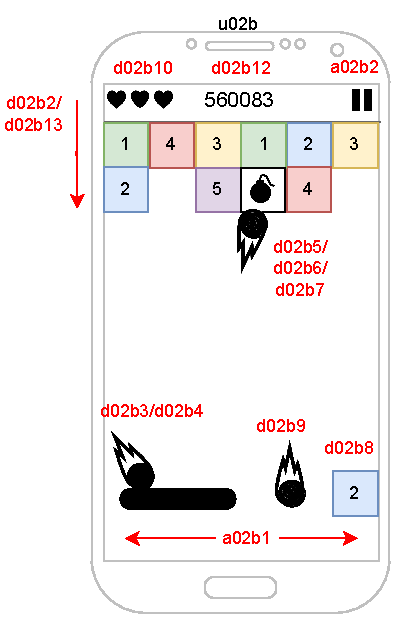
\includegraphics[scale=1.4]{diagramme/pdf/Mockup-u02b.pdf}
    \end{center}
    \caption{Dialog u02b - Spiel Invasion}\label{fig:dia:u02b}
\end{figure}

Bei dem optionalen Spielmodus \gls{invasionMode} können neben den UI-Elementen aus Dialog u02a noch die Spielmodus spezifischen Elemente auftauchen. 
Hierbei handelt es sich um Blöcke, welche zerstört werden können. Hierbei können die Blöcke unterschiedliche Stärken besitzen. 
Die Stärke repräsentiert die Anzahl an \gls{ball}berührungen, die es benötigt um einen Block zu zerstören. Außerdem können Power-Up Blöcke
erscheinen, welche dem \gls{spieler} temporäre Vorteile verschaffen können. Berührt ein Block den unteren Rand des Bildschirms, so muss das Spiel ebenfalls beendet werden (d02b8).
Wie bei dem \gls{classicMode}, muss auch hier das Spiel pausiert oder frühzeitig beendet werden können und mit der zuvor ausgewählten Schwierigkeitsstufe (leicht, mittel, schwer) initialisiert werden. Der Ball muss zu jedem Spielstart mittig des \glspl{balken} spawnen.
(siehe Fig. \ref{fig:dia:u02b})
\clearpage

\subsubsection{Dialog u09 - Sprachauswahl}\label{dialog:Sprachauswahl}

\begin{figure}[h!]
    \begin{center}
    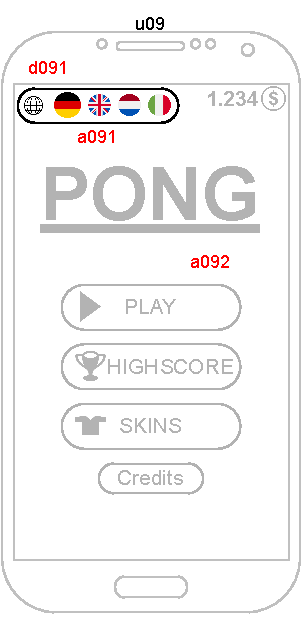
\includegraphics[scale=1.4]{diagramme/pdf/Mockup-u09.pdf}
    \end{center}
    \caption{Dialog u09 - Sprachauswahl}\label{fig:dia:u09}
\end{figure}

Bei der optionalen Sprachauswahl kann der \gls{spieler} zwischen verschiedenen Sprachen wählen und somit den im Spiel angezeigten Text entsprechend der Auswahl übersetzen lassen.
Die Flaggen repräsentieren hierbei die jeweilige Landessprache. Während der Sprachauswahl muss der Hintergrund ausgegraut sein und durch einen Klick ausserhalb des Sprachauswahl-Bereichs wieder verlassen werden können.
(siehe Fig. \ref{fig:dia:u09})
\clearpage

\subsubsection{Dialog u10 - Pause-Menü}\label{dialog:pause}

\begin{figure}[h!]
    \begin{center}
    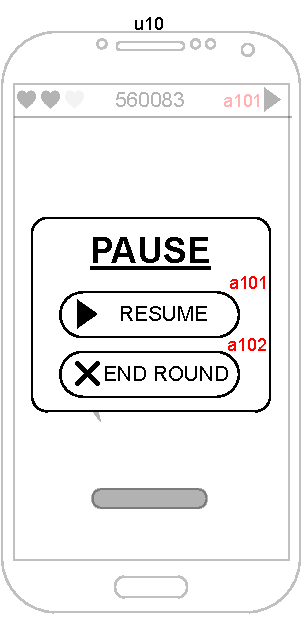
\includegraphics[scale=1.4]{diagramme/pdf/Mockup-u10.pdf}
    \end{center}
    \caption{Dialog u10 - Pause-Menü}\label{fig:dia:u10}
\end{figure}

Das Pause-Menü ist als ein Overlay über dem pausierten Spiel gestaltet und muss dem \gls{spieler} die Optionen geben, entweder das Spiel zu beenden (a102) oder das Spiel fortzusetzen (a101).
Der Hintergrund muss hierbei ausgegraut dargestellt werden.
(siehe Fig. \ref{fig:dia:u10})

\clearpage

\subsubsection{Dialog u11 - Game-Over-Menü} \label{subsec:u11-gameOverMenu}

\begin{figure}[h!]
    \begin{center}
    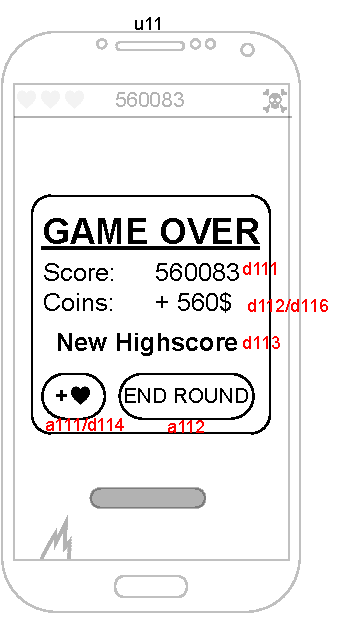
\includegraphics[scale=1.4]{diagramme/pdf/Mockup-u11.pdf}
    \end{center}
    \caption{Dialog u11 - Game-Over-Menü}\label{fig:dia:u11}
\end{figure}

Hat der \gls{spieler} keine Leben mehr, so muss der Game-Over Screen als Overlay angezeigt werden. Dieser muss dem Spieler beim ersten Mal nach jeder Spielrunde die Möglichkeit bieten eine letzte Chance zu bekommen (a111).
Diese letzte Chance muss sich durch einen Klick auf den Herz-Button auslösen lassen.
Außerdem müssen der erreichte Score (d111) und die erspielten Coins (d112) angezeigt werden.
Der \gls{spieler} muss mit einem Klick auf "End Round" (a112) zurück ins Hauptmenü geleitet werden.
Der Hintergrund muss hierbei ausgegraut dargestellt werden. 
(siehe Fig. \ref{fig:dia:u11})
\clearpage

\subsubsection{Dialog u12 - Werbung}\label{dialog:Werbung}

\begin{figure}[h!]
    \begin{center}
    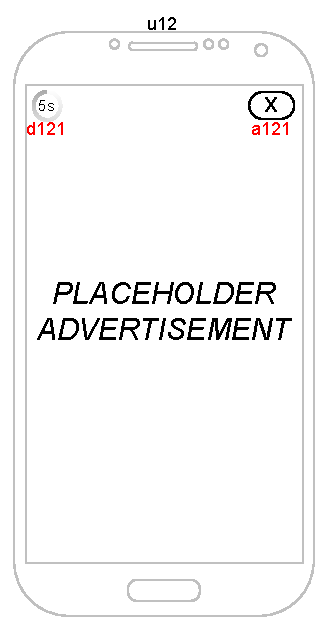
\includegraphics[scale=1.4]{diagramme/pdf/Mockup-u12.pdf}
    \end{center}
    \caption{Dialog u12 - Werbung}\label{fig:dia:u12}
\end{figure}


Entscheidet sich der \gls{spieler} dazu, Werbung anzuschauen um ein weiteres Leben zu bekommen, so wird ihm ein Werbeclip angezeigt.
Nach Ablauf der Werbung muss der \gls{spieler} diese durch einen Klick auf den X-Button beenden können (a121).
Woraufhin das Spiel mit einem letzten Leben fortgesetzt werden muss. Falls der Spieler im \gls{invasionMode} keine \gls{leben} mehr hat, muss das Spiel nach Ablauf der Werbung neu initialisiert werden. Entscheidet sich der \gls{spieler} vorzeitig dazu, dass er 
die Werbung nicht weiter schauen möchte, so muss er diese vorher beenden und somit auch den gesamten Spiel-Durchlauf beenden können (a121).
(siehe Fig. \ref{fig:dia:u12})
\clearpage

\subsubsection{Dialog u13 - Namenseingabe}\label{dialog:Namenseingabe}

\begin{figure}[h!]
    \begin{center}
    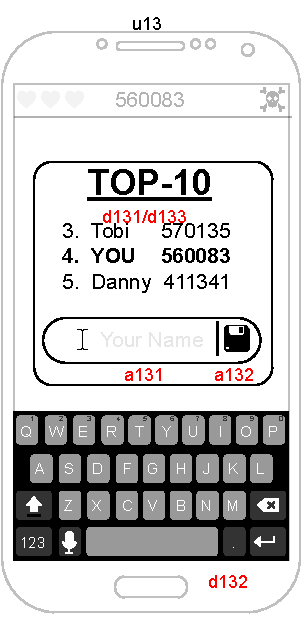
\includegraphics[scale=1.4]{diagramme/pdf/Mockup-u13.pdf}
    \end{center}
    \caption{Dialog u13 - Namenseingabe}\label{fig:dia:u13}
\end{figure}

Hat der \gls{spieler} eine \gls{Top10} Platzierung erspielt, so muss ihm seine Position in der \gls{Top10} Liste nach Ablauf der Spielrunde angezeigt werden.
Neben dem gerade erspielten Score müssen ebenfalls die zwei nächsten Scores angezeigt werden.
Der \gls{spieler} muss die Möglichkeit haben, seinen Namen einzutragen (a131) und sich mit einem Klick auf den Speichern-Button (a132) in der \gls{Top10} Liste abzuspeichern.
(siehe Fig. \ref{fig:dia:u13})
\clearpage

\subsubsection{Dialog u20 - Top-10 Liste}\label{dialog:top10}

\begin{figure}[h!]
    \begin{center}
    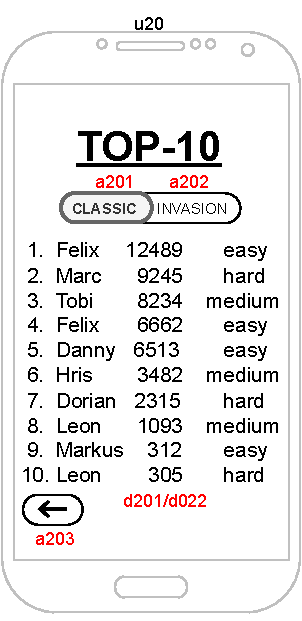
\includegraphics[scale=1.4]{diagramme/pdf/Mockup-u20.pdf}
    \end{center}
    \caption{Dialog u20 - Top-10 Liste}\label{fig:dia:u20}
\end{figure}

Die \gls{Top10} Liste muss die zehn besten Scores zeigen. Es kann für jeden Spielmodus eine einzelne Liste geben (\gls{invasionMode}, \gls{classicMode}). 
Es müssen Platzierung, Name des \glspl{spieler}, erreichte Punkte und Schwierigkeitsgrad angezeigt werden. Es soll ebenfalls die Möglichkeit geben, zwischen den \gls{Top10} Listen der jeweiligen Spielmodi wechseln zu können.
Durch einen Klick auf den Zurück-Button muss es möglich sein, zurück ins Hauptmenü zu gelangen.
(siehe Fig. \ref{fig:dia:u20})
\clearpage

\subsubsection{Dialog u25 - Achievements}\label{dialog:Achievements}

\begin{figure}[h!]
    \begin{center}
        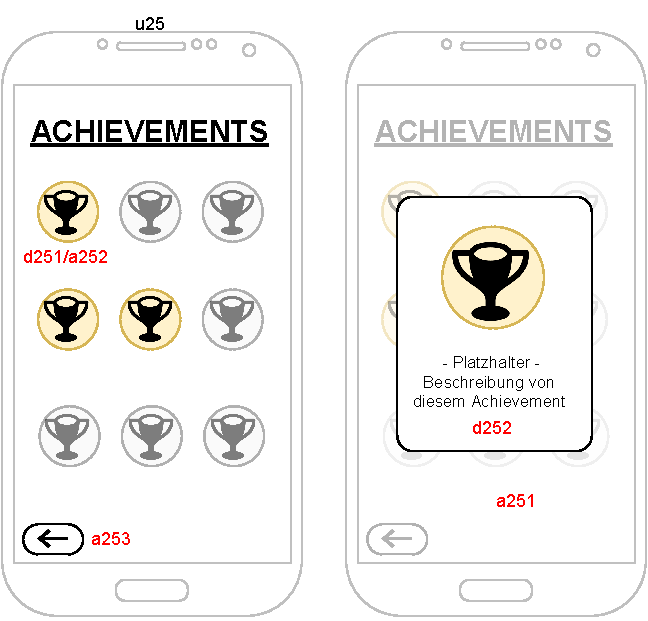
\includegraphics[scale=1.4]{diagramme/pdf/Mockup-u25.pdf}
    \end{center}
    \caption{Dialog u25 - Achievements}\label{fig:dia:u25}
\end{figure}

Auf dem Achievements Bildschirm können alle erreichbaren \gls{achievements} als Symbol dargestellt werden. Noch nicht freigeschaltete \gls{achievements} können hier ausgegraut dargestellt werden. Klickt der \gls{spieler} auf ein Achievementsymbol, kann die dazugehörige Beschreibung angezeigt werden. Ein Klick außerhalb der Beschreibung sorgt dafür, dass diese sich wieder schließt.
Dem \gls{spieler} kann es möglich sein, durch einen Klick auf den Zurück-Button wieder ins Hauptmenü zu gelangen.
(siehe Fig. \ref{fig:dia:u25})
\clearpage

\subsubsection{Dialog u30 - Skin-Auswahl}\label{dialog:skins}

\begin{figure}[h!]
    \begin{center}
    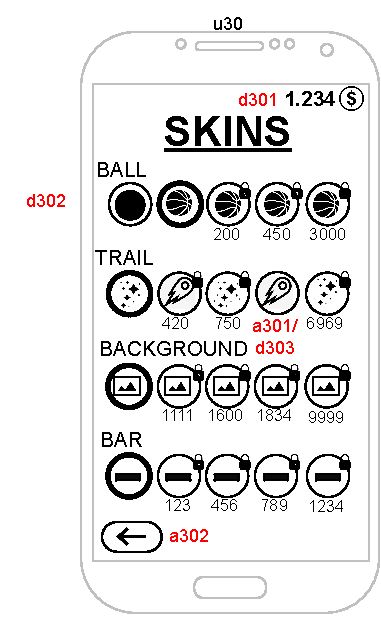
\includegraphics[scale=1.4]{diagramme/pdf/Mockup-u30.pdf}
    \end{center}
    \caption{Dialog u30 - Skin-Auswahl}\label{fig:dia:u30}
\end{figure}

Die Skin-Auswahl muss dem \gls{spieler} fünf Skins bieten, jeweils für den \gls{ball}, den Schweif, den Hintergrund und den \gls{balken}.
Dem \gls{spieler} muss es möglich sein, durch einen Klick auf den Zurück-Button wieder ins Hauptmenü zu gelangen.
Außerdem muss der \gls{spieler} sein aktuelles \gls{coin}-Guthaben in der rechten oberen Ecke angezeigt bekommen.
(siehe Fig. \ref{fig:dia:u30})
\clearpage

\subsubsection{Dialog u31 - Skin-Kauf}\label{dialog:skinkauf}

\begin{figure}[h!]
    \begin{center}
    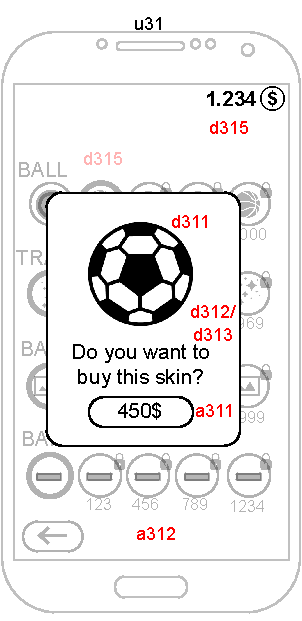
\includegraphics[scale=1.4]{diagramme/pdf/Mockup-u31.pdf}
    \end{center}
    \caption{Dialog u31 - Skin-Kauf}\label{fig:dia:u31}
\end{figure}

Kauft der \gls{spieler} einen Skin, so muss der Skin in einem Overlay vergrößert angezeigt werden. Außerdem muss der Preis angezeigt werden.
Der Hintergrund muss ausgegraut dargestellt werden und der \gls{spieler} muss sein aktuelles \gls{coin}-Guthaben in der rechten oberen Ecke angezeigt bekommen.
(siehe Fig. \ref{fig:dia:u31})
\clearpage

\subsubsection{Dialog u40 - Credits}\label{dialog:credits}

\begin{figure}[h!]
    \begin{center}
    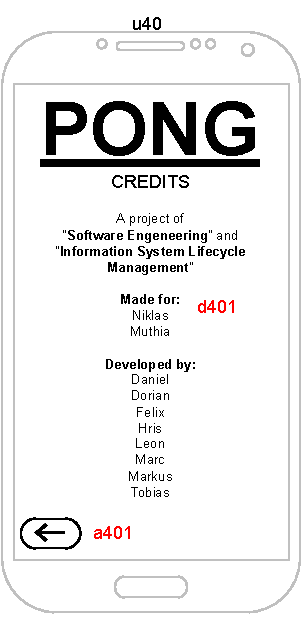
\includegraphics[scale=1.4]{diagramme/pdf/Mockup-u40.pdf}
    \end{center}
    \caption{Dialog u40 - Credits}\label{fig:dia:u40}
\end{figure}

Der \gls{spieler} muss die Möglichkeit haben in den Credits genauere Informationen zum Entwicklerteam und zur App allgemein zu bekommen.
Durch einen Klick auf den Zurück-Button, muss der \gls{spieler} wieder ins Hauptmenü gelangen.
(siehe Fig. \ref{fig:dia:u40})
\clearpage
